\documentclass{article}
\usepackage[utf8]{inputenc}
\usepackage{graphicx}
\graphicspath{{./images}}

\title{CS 250 Study Guide}
\author{Lance Ma}
\date{October 2022}

\begin{document}

\maketitle

\section{9.1 Assembly Language}

\begin{itemize}
    \item Low level language
    
    \item Few abstractions
\end{itemize}


\subsection{Assembly Language Syntax}

\textbf{Label: OpCode: Operand 1: Operand 2: Comment}

\textbf{Label}: symbolic to this instruction, allows you to refer back to it like for if statments/loops

\textbf{OpCode}: Tells the machine what operation this instruction is performing

\textbf{Opcode 1/2}: Points to where operators are being stored 

\textbf{Comment}: to tell you what this machine instruction does

\subsection{Registers}

\begin{itemize}
    \item Registers store memory/data
    \item Examples for regiter names: R10, \$3 
\end{itemize}

\subsection{Control Flow}
\begin{itemize}
    \item Need to add \textbf{offset} to default next instruction pointer to achieve control flow
    
    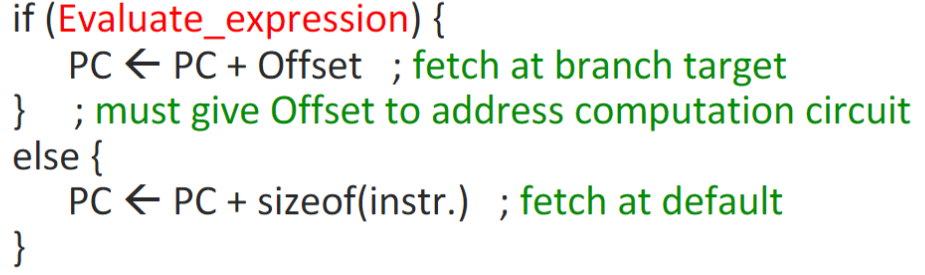
\includegraphics[scale=0.35]{images/slide1.png}
    
    \textbf{If Statement in assembly language}
    
    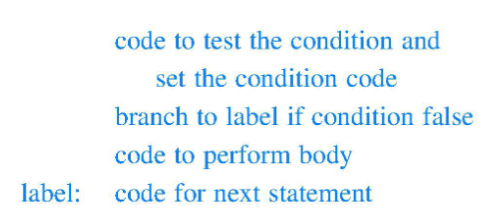
\includegraphics[scale=0.4]{images/if.png}
    
    \textbf{For loop in assembly language}
    
    \textbf{While loop in assembly language}
   
\end{itemize}

\subsection{Two Passes}
\begin{itemize}
    \item The first pass stores label names into a symbolic table
    \item Second pass replaces mnemonics with bit strings, and fills in offsets with symbol table
\end{itemize}

\subsection{Example Assembly Code}

\section{Amdhal's Law}

\begin{itemize}
    \item Amdhal's Law models how much benefit the enhancement has to the overall runtime
    
    \begin{equation}
        Speedup_{overall}=\frac{1}{(1-f_e) + (\frac{f_e}{S_e})}
    \end{equation}
    
    \item $F_e$ is the portion of the original program is got enhanced (sped up) 
    
    \item $1 - F_e$ is the portion that the enhancement is not helping
    
    \item $S_e$ = Time to execute $f_e$ without enhancement divided by time to execute fe with enhancement
    
    \item Large $S_e$ doesn't always mean a big $F_e$
    \end{itemize}

\section{Instruction Representation}
    
    \begin{itemize}
        \item 5 fields: Some machine instructions don't use all 5
        
        
        \item $2^{opcode-field-size}$ doesn't always equal the number of available opcodes in that ISA
        
        \item If opcode isn't defined in ISA, compiler discards the machine instruction
        
    \end{itemize}
    
    \subsection{Example Machine Code}
    

    \subsection{Program Control Flow}
    
    \begin{itemize}
        \item Sequential: goes through program line by line
        
        \subsubsection{Pointer Arithmetic for sequential}
        
        \begin{itemize}
            \item CurInstrucPtr + 4 (offset for default next instruc)
        \end{itemize}
            
        
        \item Skip-ahead: executes an instruction further ahead in program (if statement)
        
        \item Skip-back: skips back to a previous instruction (loops)
    \end{itemize}
 
 \subsection{Actual Next Instruction}
 
 \begin{itemize}
     \item Things known at compile time are known \textbf{statiscally} like default next = actual next, function calls (location of label of function beginning)
     
     \item Things that aren't known at compile time are know as \textbf{dynamically} known information
     
     \item Examples include if statements, while loops, and function return calls
     
     \item Actual Next is either:
     
     Cur instruction + 4 (sequential)
     Cur instruction + constant (if statement)
     saved cur instruction + 4 (from function call return)
     
 \end{itemize}
 
 \section{Fetching Machine Instruction}
 
 \begin{itemize}
     \item Registers are known as register units aka register file
     
     \item Register size is a design choice but a good choice is register size = int size = memory address size
     
     \item Pointers to operands and results take the most amount of memory in machine instruction representation
 \end{itemize}
 
 \subsection{Operands}
 \begin{itemize}
 
 \item Machine instruction operands are located within the machine instruction, memory, and in registers
 
     \item What: Some data format's are built into the hardware like 32-bit ints. Meanwhile, some are built by software like strings and structs
     
     \item When: some values are known early - constants; meanwhile some are just known right before it is used
     
     \item Where: Operands must bus to the input of the ALU
     
     
 \end{itemize}
 
 \subsubsection{Immediate Operands}
 
 \begin{itemize}
 
 \item Fastest to access
     \item IMM: operand bit string contained in machine instruction field
     
     \item Place IMM on bus to ALU at the same time as opcode
     
     \item Downside is the size
     
     
 \end{itemize}
 
 \subsubsection{Register Operands}

\begin{itemize}
    \item Operand bit string stored in register unit 
    \item Decode operand and place on register pointer. Place that register pointer on bus to register file, and that gets sent to ALU
    \item Second fastest behind IMM
\end{itemize}

\section{Boolean Algebra}

\begin{itemize}
    \item Two element sets like \{0,1\} or \{T,F\}
    
    \item Can implement AND, OR, NOT from these two values
    
    \item Boolean algebra can only have 2 values (0,1) meanwhile electronic devices can have infinite states
    
    
\end{itemize}

\subsection{CMOS}

\begin{itemize}
    \item Most modern computers use CMOS to implement their functions
    
    \item P-Channel - denoted with a dot, and allows current to flow through when there is a low voltage (0), but doesn't permit current through when it receives a high voltage (1).
    
    \item N- channel, denoted without a dot allows current to flow when it receives a high voltage but doesn't when it receives a low voltage.
    
    \item Time it takes for it to receive input and when output changes is called \textbf{propagation delay}
    
    \item Computers built from CMOS are fast and cheap, and require little power to compute
    
    \end{itemize}


\section{Combinatorial Circuits}

\begin{itemize}
    \item Truth tables define boolean functions
    
    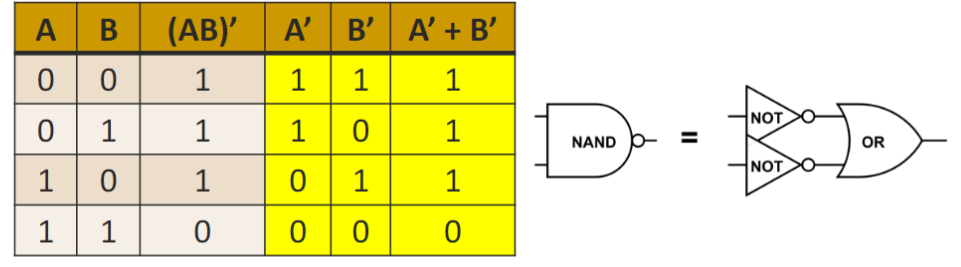
\includegraphics[scale=0.35]{images/truthtable.png}
    \item Image shows truth table for nand and it's gate equivalence
    
    
\end{itemize}
\subsection{Sum of Products}

\begin{itemize}
    \item Any boolean function can be represented with a sum of products 
    
    \item SOP has one \textbf{ANDED} term for each 1 output and oring these \textbf{minterms} give us all the 1's for this function
    
    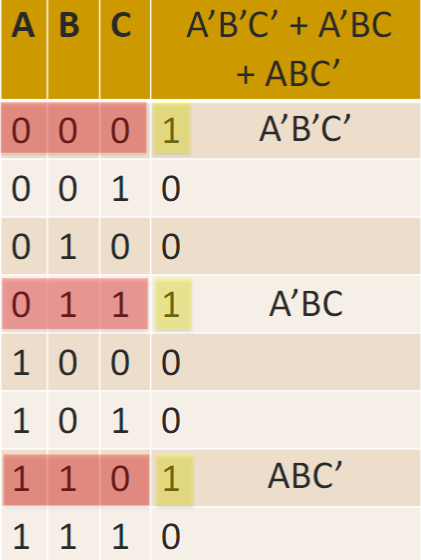
\includegraphics[scale=0.35]{images/minterms.png}
    
\end{itemize}


\subsection{Product of Sums}

\begin{itemize}
    \item If input is 1, use complement of input and or it to get all the 0's in the function
    
    \item Each sum term is a max term
    
    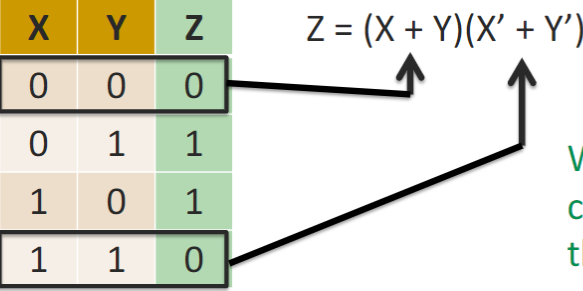
\includegraphics[scale=0.35]{images/maxterms.png}
\end{itemize}


\subsection{DeMorgan's Law and Logic Gates}

\begin{itemize}
    \item NAND is (AB) not
    
    \item written out with DeMorgan's Law is A not + B not
    
    \item NOR is (A+B) not
    
    \item written out with DeMorgan's Law is A not B not
    
    
\end{itemize}


\section{Remembering}

\begin{itemize}
    \item When a circuit's output is connected to it's input we call that \textbf{feedback}
    
    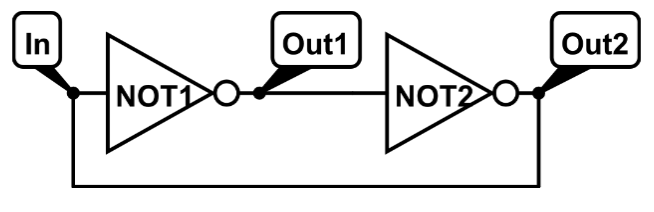
\includegraphics[scale=0.35]{images/feedback.png}
    
    \item Circuit behavior is not stable when the power is on, so sometimes it remembers a 1, sometimes a 0.
    

\end{itemize}

\subsection{Latch - SR and S'R'}

\begin{itemize}
    \item One bit memory
    
    \item Used to set or reset the output value, Q, or current state. 
    
    \item Takes 2 inputs, S and R
    
    \item SR latch is an active high and will change when it recieves a high voltage but stays the same when input stays low
    
    \item S'R' latch is an active low which changes when it receives a low voltage but stays the same when it receives a high voltage.
\end{itemize}
\end{document}
